\subsection{\label{sec:selection}Selection}
The selection operator is very useful when the user wants to obtain a subset of tuples that fulfill a certain constraint. More formally,

\begin{definition}
\label{def:crisp-selection}
 Consider the elements in definition \ref{def:valid-time-relation}.
The selection operator $\sigma$ obtains a subset of tuples that fulfill a set of constraints $P$ from an instance $r$ of the relation $R$. The set of constraints is usually a boolean combination of atomic constraints. The selection operator is noted as follows:
\end{definition}

\begin{equation}
 \label{eq:selection}
\sigma_{P} \left( r \right)
\end{equation}

Where $r \in R$ is the relation, and $P$ is the selection formula. The selection formula is a set of two elements:
% \begin{itemize}
% \item relation.attribute boolean relation relation.attribute
% \item relation.temporal-attribute allen-relation relation.temporal-attribute 
% \end{itemize}
\begin{equation}
 \label{eq:selection_formula}
P = \left \lbrace Q, Q^{T}\right \rbrace
\end{equation}

Where $Q$ is the set of non-temporal constraints and $Q^{T}$ the set of temporal constraints.
The component $Q$ is a set composed by atomic constraints: 

\begin{equation}
 \label{eq:non-temporal-constraints}
Q = \left \lbrace q_{\mbox{a}_1}  \theta \mbox{ val}_1, \ldots, q_{\mbox{a}_n}  \theta \mbox{ val}_n \right \rbrace
\end{equation}


Where:
\begin{itemize}
 \item $q_{a \in A }$ is an atomic constraint. The constraint refers to an attribute $a$ that belongs to the set of attributes $A \subseteq A_1 \ldots A_n $ of the relation $R$.
\item $\theta$ is a relational operator; usually one of $\left \lbrace =, \neq, <, \leq, >, \geq \right \rbrace$.
\item \emph{val}$_1 \ldots$\emph{val}$_n$ are values in the domain of the queried attribute. 
 \end{itemize}

The temporal constraints, $Q^t$ are provided in a similar way. The main difference is that, instead of comparisons like $\left \lbrace =, \neq, <, \leq, >, \geq \right \rbrace$, we use the Allen's relations~\cite{Allen1983}. Hence, the representation of the temporal constraints is expressed as follows:

\begin{equation}
\label{eq:temporal-constratins}
Q^{t} = \left \lbrace q_{v_1}  \AR i_1, \ldots, q_{v_n}  \AR i_n \right \rbrace
\end{equation}
Where
\begin{itemize}
\item $q_{v \in I}$ is an attribute representing a time interval. ($q_v =  \left[s_v, e_v \right]$).
\item $\AR$ is one of the thirteen Allen's relations (equal, before, overlaps, starts, finishes, meets, during) and their respective reverses (See Figure \ref{fig:allen} ).
\item $i_{x \in \left \lbrace 1 \ldots n\right \rbrace}$ is a crisp time interval with starting and ending points ($i_x = \left[s_x, e_x \right]$).

\end{itemize}

\todo[color=red!45,inline,caption={Jose:Query evaluation}]{Should we omit this part or put it in other place?}
\subsubsection{\label{crisp-query-eval}Query Evaluation}
In a crisp relational database, the modelling of the query satisfaction is a boolean result. The evaluation of the query requirements results in one of two possibilities; accept the record if it satisfies all the constraints or reject the record otherwise. The evaluation of the selection formula $P$ given in equation \eqref{eq:selection_formula} is handled as follows. For each record $r$ in the database, two things happen independently:

\begin{itemize}
 \item The crisp constraints expressed in $Q$ are evaluated and aggregated. The result of this is a boolean value. We will note as $e_Q(r)$ value for the evaluation of the constraints in  $Q$ for the record $r$.
\item The temporal constraints expressed in $Q$ are evaluated and aggregated. The result of this is again a boolean value. We will note as $e_Q^{T}(r)$ the value for the evaluation of the constraints in $Q^T$ for the record $r$.
\end{itemize}

The results from $e_Q(r)$ and $e_Q^{T}(r)$ are aggregated using a boolean combination. For valid-time intervals, the preferred combination is the \emph{'and'} ($\wedge$) operator . The function $e_{\mbox{final}}\left(r\right)$ is given by:

\begin{equation}
 \label{eq:e-final-crisp}
e_{\mbox{final}}\left(r\right) = e_Q(r) \wedge e_Q^{T}(r)
\end{equation}




% Quizás mejor dejar la agregación para el caso difuso
% In order to present the results to the user, it is necessary to provide methods for both aggregation and ranking. This is explained in the following subsection.
% 
% 
% \subsubsection{\label{crisp-ranking}Aggregation and Ranking}
% In the crisp case we need to provide a method to combine the output from $Q$ and $Q^T$. That method selects or rejects a tuple 




\begin{example}
Consider an employee's database. The data are stored in two tables; Table \ref{table:employees} ($r \in R$) contains temporal data about the employees and Table \ref{table:address} ($s \in S$) contains temporal  data about the addresses for each employee. Consider now that the user wants to obtain all the employees who are a professor and that worked in the time interval $\left[7, 10 \right]$.
%\vspace{-10pt} \ref{table:employees} \ref{table:address}

\begin{table}
\centering
\caption{Employee's table. Instance $r$ of relation $R$.}
\vspace{2mm}

\begin{tabular}{c c c c c c }
\hline
ID & Job & Works for & Start & Finish \\ \hline
1 & Professor & 4 & 5 & 10 \\
2 & Technician & 4 & 3 & 7 \\
3 & Accountant & 4  & 4 & 10 \\
4 & Administrator & - & 1 & UC \\
1 & Professor & 4 & 11 & UC \\
\hline 
\end{tabular}
\label{table:employees}

%\vspace{10pt}


\end{table}

%\vspace{-25pt}

%\vspace{-10pt}

\begin{table}
\centering
r\caption{Address table. Instance $s$ of relation $S$.}
\vspace{2mm}
\begin{tabular}{c c c c }
\hline
ID & Adr. & Start & Finish \\ \hline
1 & C/ Camino de ronda & FB & 12 \\
2 & C/ Recogidas & FB & UC \\ 
3 & C/ Pintor Maldonado & FB & UC \\
4 & C/ Mesones & FB & UC \\
1 & C/ Manuel de Falla & 12 & UC \\
\hline 
\end{tabular}
\label{table:address}

%\vspace{10pt}


\end{table}

%\vspace{-25pt}

The selection formula is the following:

\begin{equation}
 \label{eq:selection-example}
\sigma_{r.Job = 'Professor', r.\left[S, E \right] \mbox{ Contains } \left[7, 10\right]} \left(r \right)
\end{equation}
The values for $e_Q(r)$ and $e_Q^T(r)$ for each record, as well as the final aggregation (see Equation \eqref{eq:e-final-crisp}) are illustrated in Table \ref{table:crisp-intermediate-calculations-employees}.
The resultset for the selection is shown in Table \ref{table:example-selection}.
\end{example}

\begin{table}
\centering
\caption[Intermediate calculations.]{Intermediate calculations for selection formula given in equation \eqref{eq:selection-example}}
\vspace{2mm}

\begin{tabular}{c c c c c c c c }
\hline
ID & Job & Works for & Start & Finish & $e_Q(r)$& $e_Q(r)$ & $e_{final}(r)$\\ \hline
1 & Professor & 4 & 5 & 10 & True & True & True\\
2 & Technician & 4 & 3 & 7 & False & False & False\\
3 & Accountant & 4  & 4 & 10 & False & True & False\\
4 & Administrator & - & 1 & UC & False & True & False\\
1 & Professor & 4 & 11 & UC & True & False & False\\
\hline 
\end{tabular}
\label{table:crisp-intermediate-calculations-employees}

%\vspace{10pt}


\end{table}


%\vspace{-10pt}

\begin{table}
\centering
\caption{Resultset table for the selection in equation \eqref{eq:selection-example}}
\vspace{2mm}
\begin{tabular}{c c c c c c }
\hline
ID & Job & Works for & Start & Finish \\ \hline
1 & Prof. & 4 & 5 & 10 \\
\hline 
\end{tabular}
\label{table:example-selection}

%\vspace{10pt}


\end{table}

%\todo[caption={crisp cartesian product}]{Maybe the cartesian product should be inside the selection??}
\subsection{\label{sec:cartesian-product}Cartesian Product}
The relational cartesian product is defined as all the possible combinations between tuples of  $r, s$ from two given relations $R$ and $S$ respectively. It is usually noted as $r \times s$.
The temporal cartesian product operator is defined as the relational cartesian product with a predicate on the temporal valid-time intervals \cite{DengfengGao2002}. The temporal cartesian product is defined then as $r \times^T s$.

We will re-define the predicate given in \cite{DengfengGao2002} in terms of the Allen's relations. To do this, two auxiliary functions should be defined.

%\todo[caption={Crisp temporal operators}]{Instead of define inline the crisp operators for intervals, Could it be more interesting to have an appendix with the implementation?}

\begin{definition}
 \label{def:crisp-intersect}
Intersect$\left(i_1, i_2 \right)$. Given two intervals $i_1$ and $i_2$, the Intersect function returns a boolean value showing whether the two intervals intersect or not. In terms of the Allen's relations, two intervals $i_1$ and $i_2$ intersect if between them exist any of the Allen's relations except Before or After. In other words, only if the Allen's relations Before or After do not hold for the two intervals, they will intersect.

\begin{equation}
 \label{eq:crisp-intersect}
\mbox{Intersect}\left( i_1, i_2 \right) = \left \lbrace \neg \left(e_1 < s_2 \right) \vee \neg \left(e_2 < s_1 \right) \right \rbrace
\end{equation}


\end{definition}


\begin{example}
Consider the following intervals $i_1 = \left[5, 10 \right]$ and  $i_2 = \left[0, 12 \right]$. The intersect operation is calculated as follows:
\begin{align}
\mbox{Intersect}\left( i_1, i_2 \right) &=& \left \lbrace \neg \left(10 < 0 \right)  \vee \neg \left(12 < 5 \right) \right \rbrace \\
\nonumber
&=& \mbox{True} \vee \mbox{True} \\
\nonumber &=& \mbox{True}
\end{align}

\end{example}

The other auxiliary function that allows to define the predicate for the cartesian product, needs some previous definitions as well. 

\begin{definition}
 \label{def:crisp-last}
Last$\left(i_p, i_q \right)$. Given two time points $i_p$ and $i_q$, this function obtains the greatest time point.
\begin{equation}
 \label{eq:last-crisp}
\mbox{Last}\left(i_p, i_q \right) = 
\begin{cases}
i_p & \mbox{ if } i_p \mbox{ after } i_q \\
i_q & \mbox{ otherwise } 
\end{cases}
\end{equation}
Note that because both $i_p, i_q$ are time points, the after relation is implemented as $i_p > i_q$.
\end{definition}

\begin{definition}
 \label{def:crisp-first}
First$\left(i_p, i_q \right)$. Given two time points $i_p$ and $i_q$, this function obtains the least time point.
\begin{equation}
 \label{eq:first-crisp}
\mbox{First}\left(i_p, i_q \right) =
\begin{cases}
i_p & \mbox{ if } i_p \mbox{ before } i_q \\
i_q & \mbox{ otherwise } 
\end{cases}
\end{equation}
Note that because both $i_p, i_q$ are time points, the before relation is implemented as  $i_p < i_q$.
\end{definition}



\begin{definition}
 \label{def:crisp-overlapping-interval}
Overlapping-interval$\left(i_1, i_2 \right)$. Given two intervals $i_1 = \left[s_1, e_1 \right]$ and $i_2 = \left[s_2, e_2\right]$, this function returns an overlapping interval from the original two intervals.
\begin{equation}
 \label{eq:crisp-overlapping-interval}
\mbox{OvInt}\left(i_1, i_2 \right) = 
\begin{cases}
\left[\mbox{Last}\left( s_1, s_2 \right), \mbox{First}\left(e_1, e_2 \right) \right] & \mbox{ if } \mbox{Last}\left( s_1, s_2 \right) \leq \mbox{First}\left(e_1, e_2 \right) \\
\emptyset & \mbox{ otherwise } 
\end{cases}
\end{equation}
\end{definition}

Now it is possible to define the temporal cartesian product.

\begin{definition}
 \label{def:crisp-temporal-cartesian-product}
Temporal Cartesian Product. Consider the elements in definition \ref{def:valid-time-relation}.
The temporal cartesian product of two temporal relations $r \in R = \left(A_1, \ldots A_n, S, E \right)$ and $s \in S = \left(B_1 \ldots, B_m, S, E \right)$ is noted as $r \times^T s$ and is defined by the following formula:

\begin{align}
 \label{eq:crisp-temporal-cartesian-product}
r \times^T s =  \lbrace z^{\left(n+m+2 \right)} | \exists x \in r, \exists y \in s \\
\nonumber
\mbox{intersect}\left(x[S,E], y[S,E] \right) \wedge \\
\nonumber
z\left[A\right] = x\left[A\right] \wedge z\left[B\right] = y \left[B \right] \wedge \\
\nonumber
 z\left[S, E \right] = \mbox{OvInt}\left(x\left[S, E\right], y\left[S, E\right] \right) \wedge z\left[S, E\right] \neq \emptyset  \rbrace
\end{align}
Where $A$ and $B$ are a shorthand for $\left \lbrace A_1, \ldots A_n\right \rbrace$ and $\left \lbrace B_1 \ldots, B_m\right \rbrace$ respectively.
\end{definition}

The following example illustrates the temporal cartesian product.
\begin{example}
 \label{ex:crisp-temporal-cartesian-product}
Consider the employee's database mentioned before (Tables \ref{table:employees} and \ref{table:address}). Table \ref{table:example-crisp-cartesian-product} illustrates an intermediate step to compute the temporal cartesian  product.



\end{example}

\begin{table}
\begin{center}
\caption{Intermediate calculations for the temporal cartesian product.}
\vspace{2mm}
\begin{tabular}{c c c c c c c c}
\hline
r.id & s.id & $x\left[S, E\right]$ & $y\left[S, E\right]$ & $^1$ & $^2$ & $^3$  &$z\left[S, E \right]$  \\ \hline
1 & 1 & $\left[5, 10 \right]$  & $\left[FB, 11 \right]$  & True  & 11 &  5 & $\left[5, 11 \right]$ \\
1 & 2 & $\left[5, 10 \right]$  & $\left[FB, UC \right]$  & True  & UC &  5 & $\left[5, UC \right]$ \\
1 & 3 & $\left[5, 10 \right]$  & $\left[FB, UC \right]$  & True  & UC &  5 & $\left[5, UC \right]$ \\
1 & 4 & $\left[5, 10 \right]$  & $\left[FB, UC \right]$  & True  & UC &  5 & $\left[5, UC \right]$ \\
1 & 1 & $\left[5, 10 \right]$  & $\left[12, UC \right]$  & False & UC & 12 & -                     \\
2 & 1 & $\left[3, 7 \right]$   & $\left[FB, 11 \right]$  & True  & 11 &  3 & $\left[3, 11 \right]$ \\
2 & 2 & $\left[3, 7 \right]$   & $\left[FB, UC \right]$  & True  & UC &  3 & $\left[3, UC \right]$ \\
2 & 3 & $\left[3, 7 \right]$   & $\left[FB, UC \right]$  & True  & UC &  3 & $\left[3, UC \right]$ \\
2 & 4 & $\left[3, 7 \right]$   & $\left[FB, UC \right]$  & True  & UC &  3 & $\left[3, UC \right]$ \\
2 & 1 & $\left[3, 7 \right]$   & $\left[12, UC \right]$  & False & UC & 12 &  -                    \\
3 & 1 & $\left[4, 10 \right]$  & $\left[FB, 11 \right]$  & True  & 11 &  4 & $\left[4, 11 \right]$ \\
3 & 2 & $\left[4, 10 \right]$  & $\left[FB, UC \right]$  & True  & UC &  4 & $\left[4, 11 \right]$ \\
3 & 3 &  $\left[4, 10 \right]$ & $\left[FB, UC \right]$  & True  & UC &  4 & $\left[4, 11 \right]$ \\
3 & 4 & $\left[4, 10 \right]$  & $\left[FB, UC \right]$  & True  & UC &  4 & $\left[4, 11 \right]$ \\
3 & 1 & $\left[4, 10 \right]$  & $\left[12, UC \right]$  & False & 12 & 12 & -                     \\
4 & 1 & $\left[1, UC \right]$   & $\left[FB, 11 \right]$ & True  & UC &  1 & $\left[1, UC \right]$ \\
4 & 2 & $\left[1, UC \right]$   & $\left[FB, UC \right]$ & True  & UC &  1 & $\left[1, UC \right]$ \\
4 & 3 & $\left[1, UC \right]$   & $\left[FB, UC \right]$ & True  & UC &  1 & $\left[1, UC \right]$ \\
4 & 4 & $\left[1, UC \right]$   & $\left[FB, UC \right]$ & True  & UC &  1 & $\left[1, UC \right]$ \\
4 & 1 & $\left[1, UC \right]$   & $\left[12, UC \right]$ & True  & UC & 12 & $\left[12, UC \right]$ \\
1 & 1 & $\left[11, UC \right]$  & $\left[FB, 11 \right]$ & False & UC & 11 & -                      \\
1 & 2 & $\left[11, UC \right]$  & $\left[FB, UC \right]$ & True  & UC & 11 &  $\left[11, UC \right]$ \\
1 & 3 & $\left[11, UC \right]$  & $\left[FB, UC \right]$ & True  & UC & 11 & $\left[11, UC \right]$ \\
1 & 4 & $\left[11, UC \right]$  & $\left[FB, UC \right]$ & True  & UC & 11 & $\left[11, UC \right]$ \\
1 & 1 & $\left[11, UC \right]$  & $\left[12, UC \right]$ & True  & UC & 12 &  $\left[12, UC \right]$ \\
\hline 
\end{tabular}
\label{table:example-crisp-cartesian-product}
\end{center}
$^1$, intersect$\left(x\left[S, E\right], y\left[S, E\right]\right)$\\
$^2$, First$\left(x[E], y[E] \right)$ \\
$^3$, Last$\left(x[S], y[S] \right)$
\end{table}

\subsubsection{\label{sec:join}Join}
The join operator $\Join$ builds a new relation from two given relations, namely $r \in R$ and $s \in S$. This new relation is a set with all the possible combinations of tuples in both $r$ and $s$ that fulfill a predicate. It is usually noted as $r \Join_{a \theta b} s$ and called (theta) join, where $a,b$ are attributes from $r$ and $s$ respectively and $\theta$ a relational operator. The temporal join definition is based on the temporal cartesian product.

\begin{definition}
 \label{def:temporal-theta-join}
Temporal theta join. Let $r$ and $s$ be two  instances of relations $R, S$ respectively. Then the temporal theta join is defined as follows:
\begin{equation}
 \label{eq:temporal-theta-join}
r \Join_{a \theta b}^{T} s= \sigma_{a \theta b} \left(r \times^T s \right)
\end{equation}

\end{definition}


% _{\begin{figure}
%  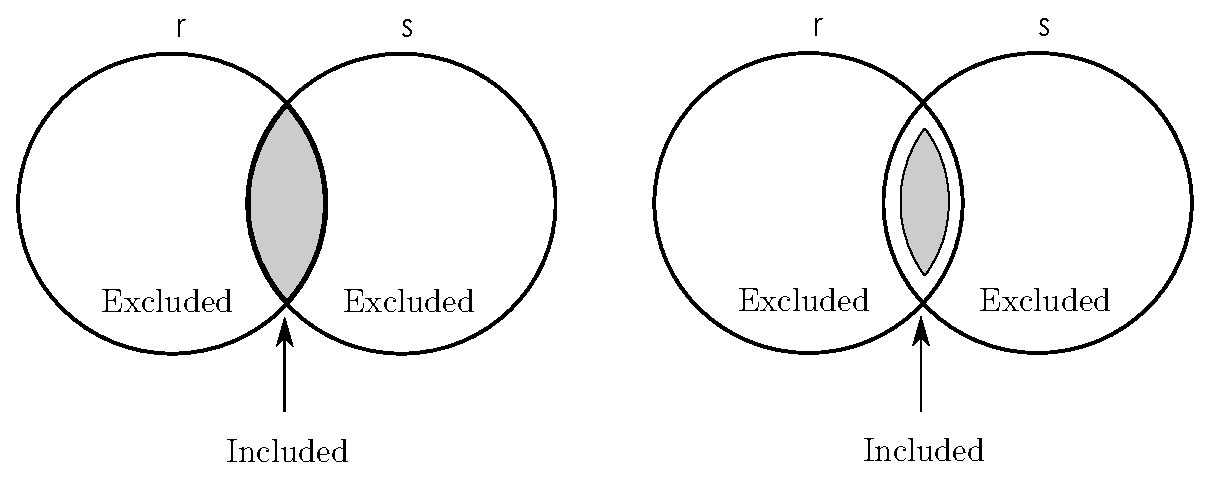
\includegraphics[scale=0.60]{graphs/innerjoin.eps}
% \caption[Comparison inner join vs temporal inner join.]{\label{fi:innerjoin} Comparison between the relational (non-temporal) inner join (left graph) and the temporal inner join (right graph).}
% \end{figure}
% 
% 
% 
% Figure \ref{fi:innerjoin} compares the relational inner join with respect to the temporal inner join. The right graph illustrates the temporal case. It is clear that the temporal inner join is a subset or is equal to the relational inner join.}

% \subsubsection{\label{subsec:Equijoin}Equijoin}
% The equijoin operator for relational databases enforces equality between specified subsets of the attributes of the relations. Then, the temporal equijoin operator is defined as the temporal join operator.
% 
% \begin{definition}
%  \label{def:equijoin}
% Equijoin. Let $R$ and $S$ be two relations and $r, s$ be the instances of each relation respectively. $A , B$ are the sets of the attributes for the relations $R$ and $S$ respectively. And let $A' \subseteq A$ and $B' \subseteq B$. Then, the temporal equijoin is defined as follows:
% \begin{equation}
%  \label{eq:equijoin}
% r \Join_{r\left[A' \right] = s\left[B' \right]}^{T} s =  \sigma_{r\left[A' \right] = s\left[B' \right]} \left(r \times^T s \right)
% \end{equation}
% \end{definition}
% 
% 
% \subsubsection{\label{subsubsec:temporal-equijoin}Temporal Equijoin}
% The temporal equijoin is an equijoin operator in which the subset of attributes in the equijoin condition, are part of the primary key. Hence, the operator is defined as follows:
% 
% \begin{definition}
% \label{def:temporal-equijoin}
% Temporal equijoin ($r \mbox{ TE-join } s$). Let $R, S$ be two relations and $r, s$ the instances of each relation respectively. Consider that $PK$ is the primary key of both relations. The temporal equijoin operator is defined as follows:
% \begin{equation}
%  \label{eq:temporal-equijoin} 
% r \mbox{ TE-join } s \equiv r \Join_{r\left[PK\right] = s\left[PK\right]}^{T} s
% \end{equation}
% \end{definition}
% 
% \subsubsection{\label{subsec:natural-join}Natural Join}
% The temporal natural join is a temporal equijoin on identically named attributes.
% 
% \begin{definition}
%  \label{def:temporal-natural-join}
% Temporal natural join. Consider the following relations $R = \left(A_1, \ldots, A_n, C_1, \ldots, C_k, S, E \right)$ and $S = \left(B_1, \ldots, B_m, C_1, \ldots, C_k, S, E \right)$. Let $r,s$ be instances of $R, S$ respectively. The temporal natural join is defined as follows:
% \begin{equation}
%  \label{eq:temporal-natural-join}
% r \Join^T s = r \Join_{r\left[C_1\right] = s\left[C_1\right] \wedge \ldots \wedge r\left[C_k\right] = s\left[C_k\right]} s
% \end{equation}
% \end{definition}

% \todo[caption={outer-joins}]{Still have to define the outer joins implementation...}
% \subsubsection{\label{subsec:outer-joins}Outer Joins}
% 
% 
% \begin{figure}
%  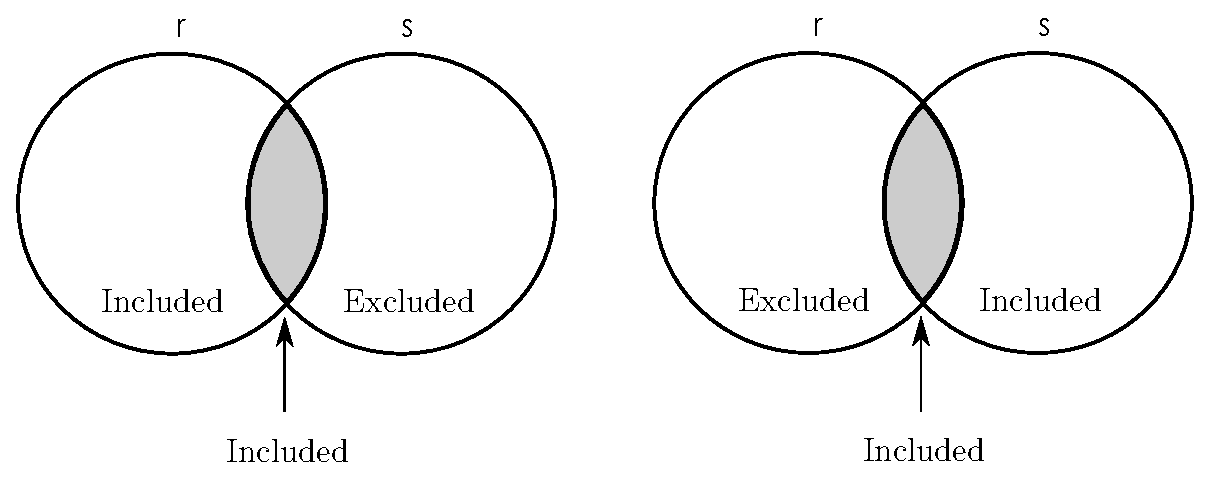
\includegraphics[scale=0.60]{graphs/outerjoin.eps}
% \caption{\label{fi:outerjoin} Comparison between a left outer join (left graph) and a right inner join (right graph).}
% \end{figure}


\subsection{Projection}
\subsection{Cartesian Product}
\subsection{Union}
\subsection{Difference}
\subsection{Intersection}
\subsection{Join}
\subsection{Division}